%%----------------------------------------------------------------------------
%% Onderzoekstechnieken: Analyse van 2 kwalitatieve variabelen
%%----------------------------------------------------------------------------

\documentclass[aspectratio=169]{beamer}

%==============================================================================
% Aanloop
%==============================================================================

%---------- Vormgeving --------------------------------------------------------

\usetheme{hogent}

\usecolortheme{hgwhite} % witte achtergrond, zwarte tekst

\usepackage{graphicx,multicol}
\usepackage{comment,enumerate,hyperref}
\usepackage{amsmath,amsfonts,amssymb}
\usepackage[dutch]{babel}
\usepackage{multirow}
\usepackage{eurosym}
\usepackage{listings}
\usepackage{textcomp}
\usepackage{framed}
\usepackage{wrapfig}
\usepackage{tabu} %needed for \tabulinesep
\usepackage{wrapfig}
\usepackage{pgf-pie}
\usepackage{pgfplots}
\usepackage{booktabs}
\usepackage{pgfplotstable}
\usepackage{changepage}
\usepackage{ulem} % for \sout{text} (strikethrough)
\usepackage{fancyvrb} % for \begin{Verbatim} (LaTeX controls within verbatim)

%---------- Configuratie ------------------------------------------------------

\pgfplotsset{compat=1.16}
\usetikzlibrary{arrows,shapes,backgrounds,positioning,shadows}
\usetikzlibrary{pgfplots.statistics}

%---------- Commando-definities -----------------------------------------------

\newcommand{\tabitem}{~~\llap{\textbullet}~~}
\newcommand{\alertbox}[2][hgblue]{%
  \setbeamercolor{alertbox}{bg=#1,fg=white}
  \begin{beamercolorbox}[sep=2pt,center]{alertbox}
    \textbf{#2}
  \end{beamercolorbox}
}
\pgfmathdeclarefunction{gauss}{2}{%
  \pgfmathparse{1/(#2*sqrt(2*pi))*exp(-((x-#1)^2)/(2*#2^2))}%
}

%---------- Info over de presentatie ------------------------------------------

\title{Hst 6. Analyse van 2 (kwalitatieve) variabelen}
\subtitle{Onderzoekstechnieken}
\author{Jens Buysse \and Wim {De Bruyn} \and Bert {Van Vreckem} \and Pieterjan Maenhaut}
\date{AJ 2020-2021}

%==============================================================================
% Inhoud presentatie
%==============================================================================

\begin{document}

\begin{frame}
  \maketitle
\end{frame}

\begin{frame}
  \frametitle{What's on the menu today?}
  
  \tableofcontents
\end{frame}

\begin{frame}
  \frametitle{Leerdoelen}
  
  \begin{itemize}
    \item Afhankelijke/onafhankelijke variabele
    \item Voor elk meetniveau geschikte analysetechnieken kunnen toepassen
    \item Kruistabellen en Cramér's $V$
    \item Visualisatie
  \end{itemize}
\end{frame}

\begin{frame}
  \frametitle{Overzicht}
    \centering
    \begin{tabular}{lll}
    	\toprule
    	\textbf{Onafhankelijke} & \textbf{Afhankelijke} & \textbf{Toets/metriek}        \\
    	\midrule
    	Kwalitatief             & Kwalitatief           & $\chi^2$-toets                \\
    	                        &                       & Cramér's $V$                  \\
    	Kwalitatief             & Kwantitatief          & $t$-toets voor 2 steekproeven \\
    	                        &                       & Cohen's $d$                   \\
    	Kwantitatief            & Kwantitatief          & ---                           \\
    	                        &                       & Regressie, correlatie         \\
    	\bottomrule
    \end{tabular}
\end{frame}

\section{Bivariate analyse}

\begin{frame}
  \frametitle{Bivariate Analyse}
  \note{Deze slide wordt gebruikt om een voorbeeld te geven van een minder triviaal verband tussen variabelen: Ant Colony optimization. Verbanden tussen variabelen zouden dus kunnen zijn:
    
    \begin{itemize}
      \item Aantal obstakels tussen nest en voedeselbron
      \item Algoritme gebruikt om feromonen weg te nemen / te plaatsen
      \item Vorm van de obstakels tussen nest en voedselbron
      \item \dots
  \end{itemize}}
  \begin{figure}
    \centering
    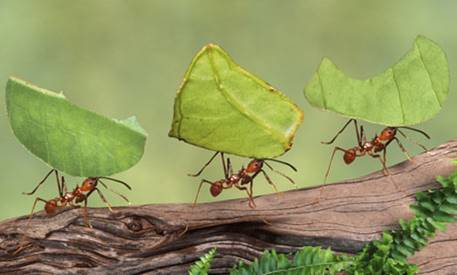
\includegraphics[width=0.8\textwidth]{ants.jpg}
    \label{fig:ants}
  \end{figure}
  
\end{frame}

\begin{frame}
  \frametitle{Voorbeeld}
  \framesubtitle{Tevredenheidsonderzoek campusrestaurant}
  
  \begin{itemize}
    \item Hoe vaakt bezoekt men het restaurant?
    \item Is er een verschil in uitgaven tussen student en medewerker?
    \item Is er een verband tussen het aantal dagen dat men bezoekt en bedrag dat men wekelijks besteedt?
  \end{itemize}
  
  R Code: zie \texttt{cursus/data/catering\_hogeschool.R}
  
  \centering
  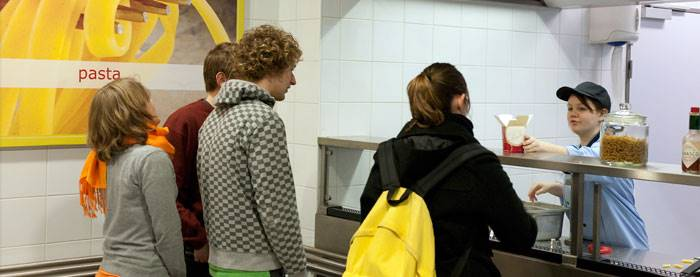
\includegraphics[height=.4\textheight]{students.jpg}
\end{frame}

\begin{frame}{Hoe vaakt bezoekt men het restaurant?}
  \begin{columns}
    \begin{column}{0.5\textwidth}
      \begin{table}[h]
        \small
        \begin{tabular}{|l|l|}
          \hline
          { \textbf{Statistiek}} & \textbf{Waarde} \\ \hline
          Mean                   & 2.96            \\ \hline
          Median                 & 3               \\ \hline
          Mode                   & 2               \\ \hline
          Stdev                  & 1.484           \\ \hline
          Variantie              & 2.202           \\ \hline
          Range                  & 4               \\ \hline
          $Q_{1}$                & 2               \\ \hline
          $Q_{2}$                & 3               \\ \hline
          $Q_{3}$                & 5               \\ \hline
        \end{tabular}
      \end{table}
    \end{column}
    \begin{column}{0.5\textwidth}
      
      \begin{figure}
        \centering
        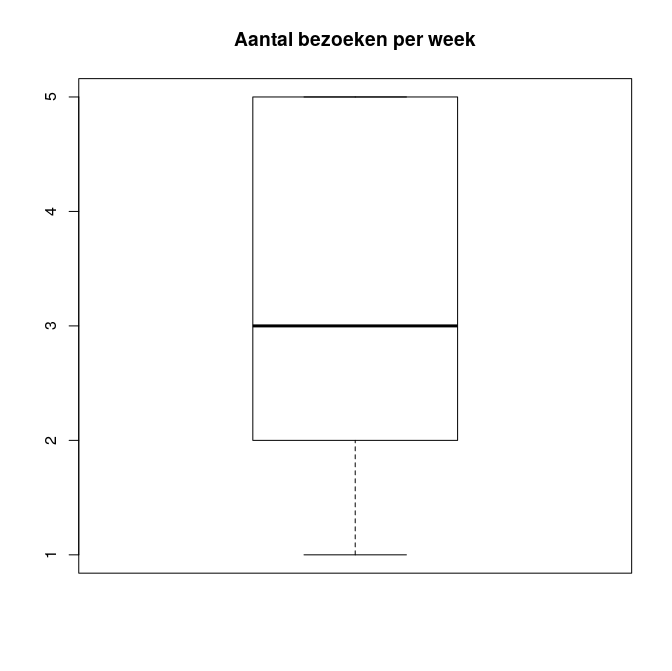
\includegraphics[height=.8\textheight]{2var-boxplot-aantalbezoeken}
        \label{fig:boxplotStudenten}
      \end{figure}
      
    \end{column}
  \end{columns}
\end{frame}

\begin{frame}{Hoe vaakt bezoekt men het restaurant?}
  
  \begin{columns}
    
    \begin{column}{0.5\textwidth}
      \begin{figure}
        \centering
        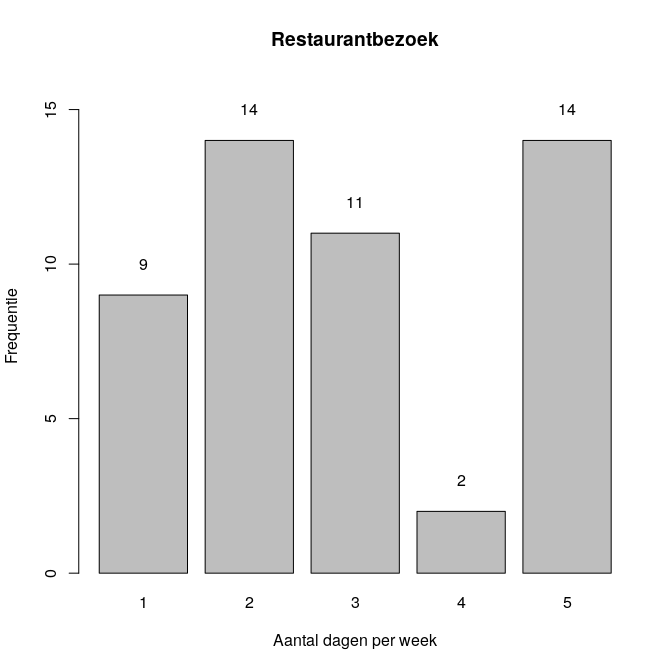
\includegraphics[height=.8\textheight]{2var-barplot-aantalbezoeken}
        \label{fig:studentenbar}
      \end{figure}
    \end{column}
    
    \begin{column}{0.5\textwidth}
      \begin{figure}
        \centering
        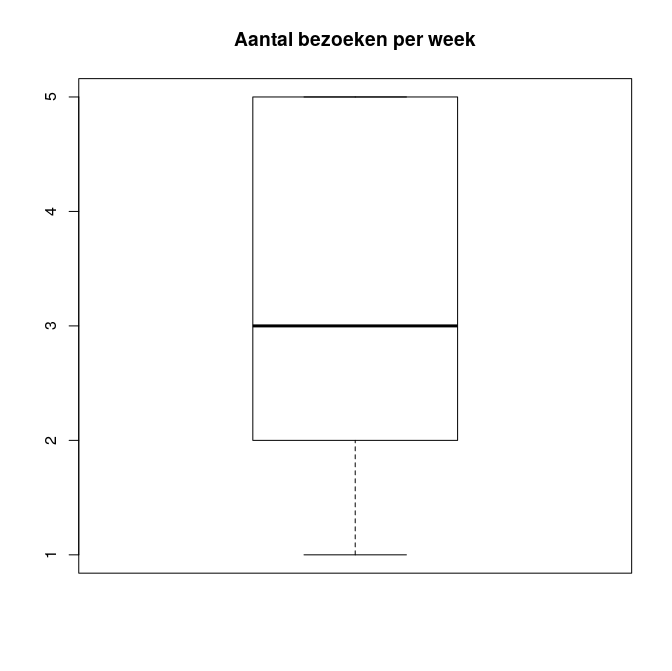
\includegraphics[height=.8\textheight]{2var-boxplot-aantalbezoeken}
        \label{fig:boxplotStudenten2}
      \end{figure}
    \end{column}
    
  \end{columns}
\end{frame}

\begin{frame}{Student vs werknemer}
  
  \begin{itemize}
    \item \alert<1>{Enkelvoudig staafdiagram} (van gemiddelde per categorie)
    \item \alert<2>{Boxplot}
  \end{itemize}
  
  \begin{figure}
    \centering
    \only<1>{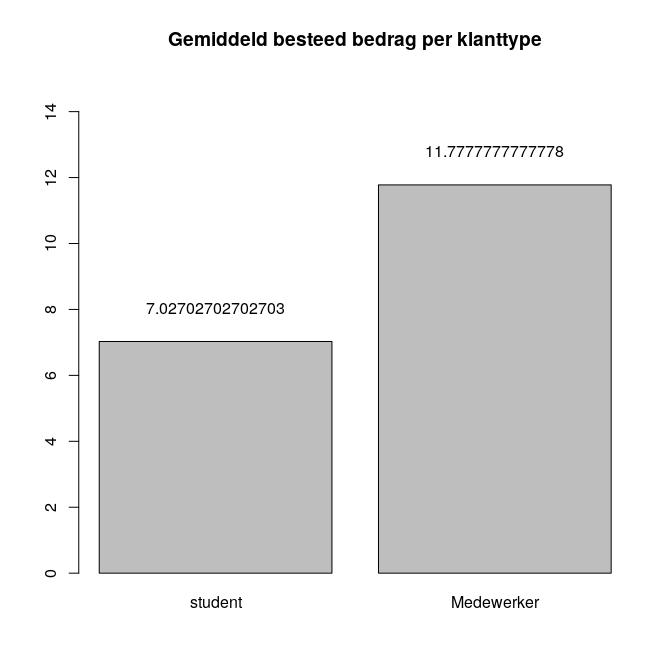
\includegraphics[height=0.6\textheight]{2var-barplot-gemiddeld-bedrag}}
    \only<2>{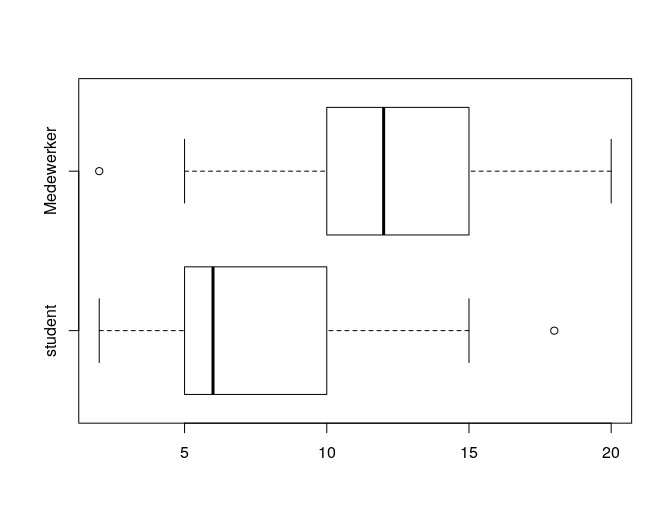
\includegraphics[height=0.6\textheight]{2var-boxplot-klanttype-bedrag}}
  \end{figure}
  
  \only<1>{\textbf{Let op!} Onvoldoende om significant verschil aan te tonen!}
\end{frame}

\begin{frame}
  \frametitle{Afhankelijke en onafhankelijke variabele}
  
  \begin{columns}
    \begin{column}{0.3\textwidth}
      
      \begin{figure}
        \centering
        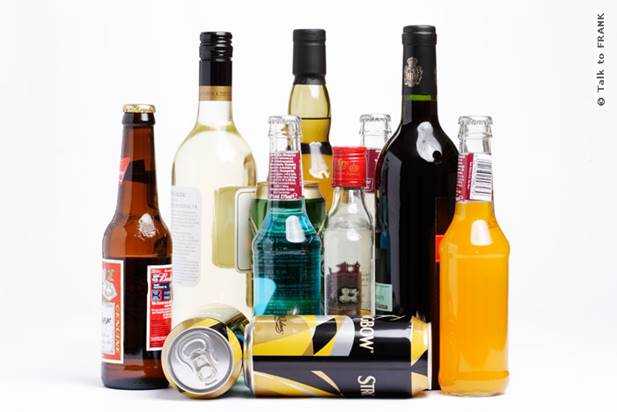
\includegraphics[width=1.00\textwidth]{liquor.jpg}
        \label{fig:liquor}
      \end{figure}
      
    \end{column}
    \begin{column}{0.3\textwidth}
      
      \begin{figure}
        \centering
        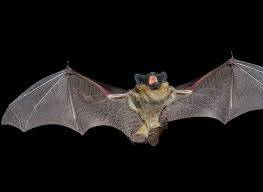
\includegraphics[width=1.00\textwidth]{bat.jpg}
        \label{fig:bat}
      \end{figure}
      
    \end{column}
    \begin{column}{0.3\textwidth}
      
      \begin{figure}
        \centering
        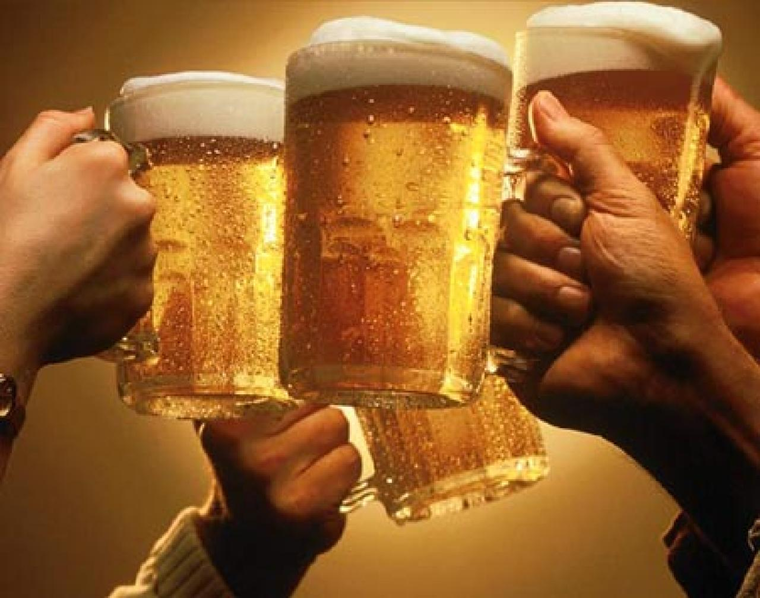
\includegraphics[width=1.00\textwidth]{beer.png}
        \label{fig:beer}
      \end{figure}
      
    \end{column}
  \end{columns}
  \note{Onderzoeken die hier gevoerd zijn:
    
    \begin{itemize}
      \item Invloed van alcoholinname op leervermogen van vleermuizen (Drinking and Flying: Does Alcohol Consumption Affect the Flight and Echolocation Performance of Phyllostomid Bats?)
      \item Arnd Leike of the Ludwig Maximilians University receives one of the Ig Nobel awards - which are given for research that cannot or should not be repeated - for demonstrating that beer froth obeys the mathematical law of exponential decay.
  \end{itemize}}
\end{frame}

\begin{frame}
  \frametitle{Onderzoek academiejaar 2013-2014}
  \begin{columns}
    \begin{column}{0.3\textwidth}
      
      \begin{figure}
        \centering
        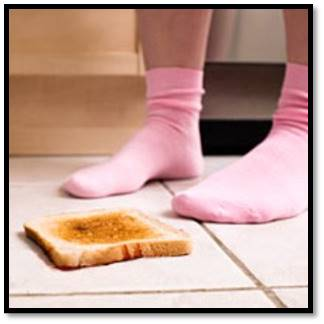
\includegraphics[width=1.00\textwidth]{toast.jpg}
        \label{fig:toast}
      \end{figure}
      
    \end{column}
    \begin{column}{0.3\textwidth}
      
      \begin{figure}
        \centering
        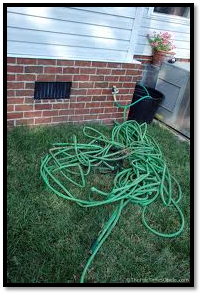
\includegraphics[width=1.00\textwidth]{hose.png}
        \label{fig:hose}
      \end{figure}
      
    \end{column}
    \begin{column}{0.3\textwidth}
      
      \begin{figure}
        \centering
        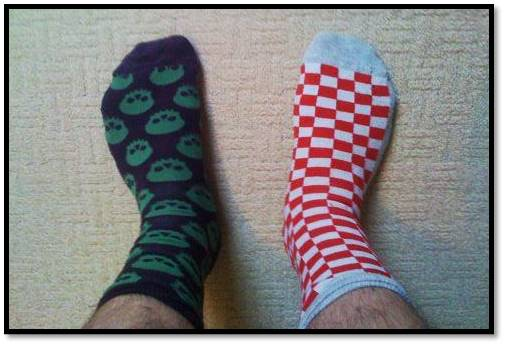
\includegraphics[width=1.00\textwidth]{socks.jpg}
        \label{fig:socks}
      \end{figure}
      
    \end{column}
  \end{columns}
  \note{Studenten moesten onderzoeken of er een verband was tussen vallen van boterham op boterzijde en hoogte e.a., of verband was tussen het aantal onpare sokken en andere fenomenen zoals je eigen was doen, veel sporten al dan niet \dots}
\end{frame}

\section{Kruistabellen en Cramér's V}

\begin{frame}
  \frametitle{Kruistabellen}
  Is er een verschil in waardering in het assortiment tussen mannen en vrouwen?
  
  \begin{table}[h]
    \begin{tabular}{l||l|l||l}
      & Vrouw & Man & Totaal \\ \hline \hline
      Goed        & 9     & 8   & 17     \\
      Voldoende   & 8     & 10  & 18     \\
      Onvoldoende & 5     & 5   & 10     \\
      Slecht      & 0     & 4   & 4      \\ \hline \hline
      Totaal      & 22    & 27  & 49     \\
    \end{tabular}
  \end{table}
\end{frame}

\begin{frame}
  \frametitle{Chi-kwadraat ($\chi^2$) }
  
  \alertbox{Chi-kwadraat ($\chi^2$) is een metriek die aangeeft hoeverre de waarden in een kruistabel afwijken van de verwachte waarden als je veronderstelt dat er \textit{geen} verband is tussen twee variabelen.}
  
  \[ \chi^2 = \sum \frac{(o - e)^2}{e} \]
  
  \begin{itemize}
    \item De som wordt berekend over alle cijfers in een kruistabel
    \item $o$: geobserveerde waarde
    \item $e$: verwachte waarde
  \end{itemize}
\end{frame}

\begin{frame}
  \frametitle{Kruistabellen}
  \framesubtitle{Percenteren}
  
  \begin{adjustwidth}{-1.5em}{-1.5em}
    \begin{table}[h] \centering
      \begin{tabular}{@{}rrrrrrr@{}} \toprule
        & Vrouw & Man & Totaal & Vrouw \% & Man\%   & Totaal  \\ \midrule
        Goed        & $9$     & $8$  & $17$     & $41$\%  & $30$\%  & $35$\% \\
        Voldoende   & $8$     & $10$ & $18$     & $36$\%  & $37$\%  & $37$\% \\
        Onvoldoende & $5$     & $5$  & $10$     & $23$\%  & $18$\%  & $20$\% \\
        Slecht      & $0$     & $4$  & $4$      & $0$\%   & $15$\%  & $8$\%  \\
        Totaal      & $22$    & $27$ & $49$     & $100$\% & $100$\% & $100$\%\\
        \bottomrule
      \end{tabular}
    \end{table}
  \end{adjustwidth}
\end{frame}

\begin{frame}
  \frametitle{Kruistabellen}
  \framesubtitle{Verschil bepalen $(o - e)$}
  
  \begin{adjustwidth}{-1.5em}{-1.5em}
    \begin{table}[h] \centering
      \begin{tabular}{@{}rrrrrrr@{}} \toprule
        & Vrouw & Man & Totaal & Vrouw \% & Man\%   & Totaal  \\ \midrule
        Goed        & $9 -\textcolor{red}{7.63}$     & $8 - \textcolor{red}{9.36}$   & $17$     & $41$\%  & $30$\% & $35$\% \\
        Voldoende   & $8 - \textcolor{red}{8.08}$   & $10 - \textcolor{red}{9.91}$  & $18$     & $36$\%  & $37$\%    & $37$\% \\
        Onvoldoende & $5 - \textcolor{red}{4.48}$    & $5 - \textcolor{red}{5.51}$  & $10$     & $23$\%  & $18$\% & $20$\% \\
        Slecht      & $0 - \textcolor{red}{1.79}$    & $4 - \textcolor{red}{2.20}$  & $4$      & $0$\%      & $15$\% & $8$\%  \\
        Totaal      & $22$    & $27$  & $49$     & $100$\%    & $100$\%   & $100$\%   \\
        \bottomrule
      \end{tabular}
    \end{table}
  \end{adjustwidth}
\end{frame}

\begin{frame}
  \frametitle{Kruistabellen}
  \framesubtitle{Kwadrateren en normaliseren $\frac{(o-e)^2}{e}$}
  
  \begin{table}[h] \centering
    \begin{tabular}{@{}rrrrrrr@{}} \toprule
      & Vrouw                   & Man                     & Totaal & Vrouw \% & Man\%   & Totaal  \\
      \midrule
      Goed        & $\textcolor{blue}{0.2}$ & $\textcolor{blue}{0.2}$ & $17$   & $41$\%   & $30$\%  & $35$\% \\
      Voldoende   & $\textcolor{blue}{0}$   & $\textcolor{blue}{0}$   & $18$   & $36$\%   & $37$\%  & $37$\% \\
      Onvoldoende & $\textcolor{blue}{0.1}$ & $\textcolor{blue}{0}$   & $10$   & $23$\%   & $18$\%  & $20$\% \\
      Slecht      & $\textcolor{blue}{1.8}$ & $\textcolor{blue}{1.5}$ & $4$    & $0$\%    & $15$\%  & $8$\%  \\
      Totaal      & $22$                    & $27$                    & $49$   & $100$\%  & $100$\% & $100$\%   \\
      \bottomrule
    \end{tabular}
  \end{table}
  \[ \chi^{2} = 3.811, V= 0.279 \]
\end{frame}

\section{Cramér's V}

\begin{frame}
  \frametitle{Cramér's V}
  
  \alertbox{Cramér's V is een maat die aanduidt hoe sterk de samenhang is tussen twee kwalitatieve variabelen. Dit getal ligt altijd tussen 0 en 1}
  
  \[ V = \sqrt{\frac{\chi^2}{n (k - 1)}} \]
  
  $n$: het aantal waarnemingen
  
  $k$: min(aantal rijen, aantal kolommen)
\end{frame}

\begin{frame}
  \frametitle{Interpretatie Cramér's V}
  
  \begin{table}[h] \centering
    \begin{tabular}{@{}rr@{}} \toprule
      Waarde & Interpretatie \\
      \midrule
      $0$ & geen samenhang \\
      $0.1$ &  zwakke samenhang \\
      $0.25$ & redelijk sterke samenhang \\
      $0.5$ & sterke samenhang \\
      $0.75$ & zeer sterke samenhang \\
      $1$ & volledige samenhang \\
      \bottomrule
    \end{tabular}
  \end{table}
\end{frame}

\begin{frame}
  \frametitle{Voorbeeld 2}
  \framesubtitle{Verband tussen geslacht en voorkeur automerk}
  
  \begin{table}[h] \centering
    \begin{tabular}{@{}rrrrrr@{}} \toprule
      & Mercedes & BMW & Porsche& Alfa Romeo & Totaal \\
      \midrule
      Mannen  & $10$ & $10$ & $20$ & $20$ & $60$ \\
      Vrouwen & $20$ & $5$  & $15$ & $0$  & $40$ \\
      Totaal  & $30$ & $15$ & $35$ & $20$ & $100$ \\
      \bottomrule
    \end{tabular}
  \end{table}
  Het lijkt alsof de automerken niet gelijkelijk gewaardeerd worden door mannen en vrouwen.
  \[ \chi^{2} = 22.619, V = \sqrt{\frac{22.169}{100 . (2-1)}}  = 0.476\]
\end{frame}


\section{Chi-kwadraattoets voor één variabele}

\begin{frame}
  \frametitle{Goodness of fit test}
  \alertbox{Een \textcolor{hgyellow}{goodness of fit test} geeft aan in welke mate een steekproef overeenstemt met een nulhypothese over de verdeling van een kwalitatieve variabele.}
  
  \begin{columns}
    \begin{column} {0.35\textwidth}
      
      \begin{figure}
        \centering
        
\includegraphics[height=.5\textheight]{les6-man.jpg}
      \end{figure}
      
    \end{column}
    \begin{column} {0.65\textwidth}
      
      \begin{figure}
        \centering
        
\includegraphics[height=.5\textheight]{les5-heroes.jpg}
      \end{figure}
      
    \end{column}
  \end{columns}
\end{frame}

\begin{frame}
  \frametitle{Goodness of fit test}
  \begin{columns}
    \begin{column} {0.2 \textwidth}
      
      \begin{figure}
        \centering
        
\includegraphics[width=\textwidth]{les6-man.jpg}
      \end{figure}
      
    \end{column}
    
    \begin{column} { 0.8 \textwidth}
      \begin{table}[h]
        \begin{tabular}{@{}lcc@{}}
          \toprule
          \textbf{Type}   & \textbf{\# steekproef} & \textbf{\# populatie} \\ \midrule
          Mutant          &          127           &         35\%          \\
          Mens            &           75           &         17\%          \\
          Alien           &           98           &         23\%          \\
          God             &           27           &          8\%          \\
          Demon           &           73           &         17\%          \\ \midrule
          \textbf{Totaal} &          400           &         100\%         \\
        \end{tabular}
      \end{table}
    \end{column}
  \end{columns}
\end{frame}

\begin{frame}
  \frametitle{Goodness of fit test}
  Is de verdeling van de steekproef ($n = 400$) representatief voor de volledige populatie (alle superhelden)?
  
  \begin{itemize}
    \item Welke aantallen zou je \textit{verwachten} als de steekproef representatief is?
    \item Hoe groot is de afwijking van de \textit{geobserveerde} aantallen?
    \begin{itemize}
      \item klein $\Rightarrow$ verdeling is representatief
      \item groot $\Rightarrow$ verdeling is \textbf{niet} representatief
    \end{itemize}
  \end{itemize}
  
  \pause
  Zie je een overeenkomst met kruistabellen en Cramer's V?
\end{frame}

\begin{frame}
  \frametitle{Notatie}
  
  In de volgende slides is:
  
  \begin{itemize}
    \item $e$ de \textit{verwachte} frequentie voor een categorie
    \item $\pi$ de verwachte \textit{relatieve frequentie} voor een categorie (percentage)
    \item $o$ de \textit{geobserveerde} absolute frequentie
    \item $n$ de steekproefgrootte (zoals steeds)
    \item $i$ een index die een categorie in de frequentietabel aanduidt ($i \in \{1, \ldots, k\}$)
  \end{itemize}
\end{frame}

\begin{frame}
  \frametitle{Goodness of fit test}
  \begin{itemize}
    \item Exact representatief $\Rightarrow$ 35\% van de superhelden in de steekproef is een mutant
    \item Het verwachte aantal is dus $e = 0.35 \times 400 = 140$.
  \end{itemize}
  Er geldt dus:
  
  \[ e = n \times \pi \]
  
  Als de verschillen $o - e$  relatief klein zijn kunnen ze toegerekend worden aan toevallige steekproeffouten.
\end{frame}

\begin{frame}
  \frametitle{Goodness of fit test}
  Beschouw $\chi^{2}$:
  
  \[ \chi^{2} = \sum_{i=1}^{n} \frac{(o_{i} - e_{i})^{2}}{e_{i}} \]
  
  Besluit op basis van de waarde van $\chi^2$:
  \begin{itemize}
    \item klein $\Rightarrow$ verdeling representatief
    \item groot $\Rightarrow$ verdeling \textbf{niet} representatief
  \end{itemize}
  
  $\chi^{2}$ meet de mate van strijdigheid met de nulhypothese
\end{frame}

\begin{frame}
  \frametitle{Goodness of fit test}
  \begin{columns}
    \begin{column} {0.2 \textwidth}
      
      \begin{figure}
        \centering
        
\includegraphics[width=\textwidth]{les6-man.jpg}
      \end{figure}
      
    \end{column}
    
    \begin{column} { 0.8 \textwidth}
      % Please add the following required packages to your document preamble:
      % \usepackage{booktabs}
      \begin{table}[h]
        \begin{tabular}{@{}llllll@{}}
          \toprule
          \textbf{Type superheld} & \textbf{$o$} & \textbf{$\pi$} & \textbf{$e$} & \textbf{$o -e$} & \textbf{$\frac{(o-e)^{2}}{e}$} \\ \midrule
          Mutant                  & 127          & 35\%           & 140          & -13             & 1.21                           \\
          Mens                    & 75           & 17\%           & 68           & 7               & 0.72                           \\
          Alien                   & 98           & 23\%           & 92           & 6               & 0.39                           \\
          God                     & 27           & 8\%            & 32           & -5              & 0.78                           \\
          Demon                   & 73           & 17\%           & 68           & 5               & 0.37                           \\ \bottomrule
        \end{tabular}
      \end{table}
    \end{column}
  \end{columns}
\end{frame}


\begin{frame}
  \frametitle{Goodness of fit test}
  
  \begin{itemize}
    \item De teststatistiek $\chi^{2}$ is verdeeld volgens de $\chi^2$ verdeling.
    \item Kritieke grenswaarde $g$ bij de $\chi^{2}$ verdeling: hierbij speel het aantal vrijheidsgraden een rol ($df$). Er geldt:
    
    \[ df = k -1 \]
    
    \item De kritieke grenswaarde $g$ voor een gegeven significantieniveau $\alpha$ en vrijheidsgraden $df$ kan berekend worden met de R-functie `qchisq()`.
    
    \[ P(\chi^2 < g) = 1 - \alpha \]
  \end{itemize}
\end{frame}

\begin{frame}[fragile]
  \frametitle{Goodness of fit test}
  \framesubtitle{Berekening kritieke grenswaarde}
  
  \begin{itemize}
    \item Stel $\alpha = 0,05$ en $df = 5 - 1 = 4$
    \item \verb|g <- qchisq(0.95, df = 4)|, dus $g = 9,49$
    \item $\chi^{2} = 3,47 < g = 9,49$
    \item Besluit: de steekproef is representatief ($H_0$ wordt aanvaard)
  \end{itemize}
\end{frame}

\begin{frame}[fragile]
  \frametitle{Goodness of fit test}
  \framesubtitle{Berekening overschrijdingskans}
  
  Je kan ook de overschrijdingskans berekenen:
  
  \[ p = P(X > \chi^2) = 1 - P(X < \chi^2) \]
  
  \begin{itemize}
    \item \verb|p <- 1 - pchisq(3.47, df = 4)|, dus $p = 0,48$
    \item $p = 0,48 < \alpha = 0,05$
    \item Besluit: de steekproef is representatief ($H_0$ wordt aanvaard)
  \end{itemize}
\end{frame}

\subsection{Toetsingsprocedure goodness of fit test}

\begin{frame}
  \frametitle{Goodness of fit test}
  \framesubtitle{Toetsingsprocedure}
  
  \begin{enumerate}
    \item \textbf{Bepalen hypotheses}
    \begin{itemize}
      \item $H_{0}$: steekproef is representatief naar populatie
      \item $H_{1}$: steekproef is niet representatief naar populatie
    \end{itemize}
    \item \textbf{Bepalen $\alpha$ en $n$} : $\alpha = 0,05$ en $n = 400$.
  \end{enumerate}
\end{frame}

\begin{frame}
  \frametitle{Goodness of fit test}
  \framesubtitle{Toetsingsprocedure}
  
  \begin{enumerate}
    \item \textbf{Toetsingsgrootheid berekenen}:
    \[ \chi^{2} = \sum_{i=1}^{n} \frac{(o_{i} - e_{i})^{2}}{e_{i}} \]
    \item 
    \begin{enumerate}
      \item \textbf{Kritiek gebied}: Bereken $g$ zodat $P(\chi^2 < g) = 1 - \alpha$
      \item \textbf{Overschrijdingskans}: Bereken $p = 1 - P(X < \chi^2)$
    \end{enumerate}
    
    \item Besluit (de toets is altijd rechtszijdig):
    \begin{enumerate}
      \item $\chi^2 < g \Rightarrow$ aanvaard $H_0$, anders verwerp $H_0$
      \item $p > \alpha \Rightarrow$ aanvaard $H_0$, anders verwerp $H_0$
    \end{enumerate}
  \end{enumerate}
\end{frame}


\subsection{Voorbeeld}

\begin{frame}
  \frametitle{Voorbeeld gezinnen}
  Beschouw alle gezinnen met 5 kinderen in een bepaalde gemeenschap.
  \pause
  Met betrekking tot samenstelling zijn er 6 mogelijkheden.
  \begin{enumerate}
    \item 5 jongens
    \item 4 jongens, 1 meisje
    \item 3 jongens, 2 meisjes
    \item 2 jongens, 3 meisjes
    \item 1 jongen, 4 meisjes
    \item 5 meisjes
  \end{enumerate}
  Het onderzoek bevat 1022 gezinnen met 5 kinderen
  \begin{center}
    Zijn de waargenomen aantallen in de 6 klassen representatief voor een populatie waar de kans om een jongen te krijgen = kans om een meisje te krijgen = 0,5?
  \end{center}
\end{frame}

\begin{frame}
  \frametitle{Voorbeeld}
  \begin{table}[h]
    \begin{tabular}{@{}llllllll@{}}
      \toprule
      i       & 0  & 1   & 2   & 3   & 4   & 5  &  \\ \midrule
      $o_{i}$ & 58 & 149 & 305 & 303 & 162 & 45 &  \\ \bottomrule
    \end{tabular}
  \end{table}
  \pause
  Indien de veronderstelling waar is wordt de kans $\pi_{i}$ om $i$ jongens te krijgen bepaald door een binominaalvedeling met parameters $n=5$ en $p=0.5$.
  Bv. De kans om 2 jongens te krijgen met 5 kinderen is gelijk aan :
  
  \[ (0.5)^{2} \times (1-0.5)^{5-2} \times \binom{5}{2} \]
  
  Algemeen geldt dus:
  
  \[ \pi_{i} = \binom{5}{i}\times 0.5^{i} \times 0.5^{5-i} = \frac{5!}{i!(5-i)!}\times 0.5^{i} \]
\end{frame}

\begin{frame}
  \frametitle{Voorbeeld}
  \begin{table}[h]
    \begin{tabular}{@{}llllllll@{}}
      \toprule
      $i$                   & 0     & 1       & 2      & 3        & 4      & 5     & Tot.  \\ \midrule
      $o_i$                 & 58    & 149     & 305    & 303      & 162    & 45    & 1022  \\
      $\pi_i$               & 0.03  & 0.15    & 0.31   & 0.31     & 0.15   & 0.031 & 1     \\
      $e_i$                 & 31.68 & 159.43  & 318.86 & 318.86   & 159.43 & 31.68 &       \\
      $\frac{(o-e)^{2}}{e}$ & 21.86 & 0.68259 & 0.60   & 0.78     & 0.041  & 5.59  & 29.57 \\
      $r_i$                 & 4.74  & -0.89   & -0.93  & -1.07106 & 0.22   & 2.40  &       \\ \bottomrule
    \end{tabular}
  \end{table}
\end{frame}

\begin{frame}
  \frametitle{Voorbeeld}
  \begin{enumerate}
    \item \textbf{Bepalen hypotheses}
    \begin{itemize}
      \item $H_{0}$: steekproef is representatief naar populatie
      \item $H_{1}$: steekproef is niet representatief naar populatie
    \end{itemize}
    \item \textbf{Bepalen $\alpha$ en $n$} : $\alpha = 0.01$ en $n = 1022$.
    \item \textbf{Toetsingsgrootheid en waarde ervan in steekproef}:
    \[ \chi^{2} = \sum_{i=1}^{n} \frac{(o_{i} - e_{i})^{2}}{e_{i}} \approx 29.5766 \]
    \item \textbf{Bereken en teken kritiek gebied}:  kritieke grens is $15.0863$. Onze toetsingsgrootheid ligt dus in het kritieke gebied dus verwerpen we $H_{0}$.
  \end{enumerate}
\end{frame}

\subsection{Gestandaardiseerde residuen}
\begin{frame}
  \frametitle{Gestandaardiseerde residuen}
  \alertbox{De \textcolor{hgyellow}{gestandaardiseerde residuen} duiden aan welke klassen de grootste bijdrage leveren aan de waarde van de grootheid. }
  \[ r_{i} = \frac{o_{i} - n \pi_{i}}{\sqrt{n \pi_{i}(1-\pi_{i})}} \]
  
  \begin{itemize}
    \item Er geldt algemeen: waarden groter dan 2 of kleiner dan $-2$ zijn extreem.
  \end{itemize}
  We kunnen dus besluiten dat het aantal gezinnen waarin alle kinderen hetzelfde geslacht hebben groter mag worden genoemd dan verwacht.
  
\end{frame}

\begin{frame}
  \frametitle{Voowaarden}
  Om de toets te mogen toepassen dient aan de volgende voorwaarden te zijn voldaan (Regel van Cochran)
  \begin{enumerate}
    \item Voor alle categorie\"en moet gelden dat de verwachte waarde $e$ groter is dan 1.
    \item In ten hoogste 20 \% van de categori\"en mag de verwachte waarde $e$ kleiner dan 5 zijn.
  \end{enumerate}
\end{frame}

\section{Chi-kwadraattoets voor twee variabelen}

\begin{frame}
  \frametitle{$\chi^{2}$ toets voor twee variabelen}
  De Chi-kwadraattoets \index{$\chi^{2}$kwadraatkruistabeltoets} laat zich eenvoudig uitbreiden tot een onderzoeksontwerp met twee variabelen, met respectievelijk $r$ en $k$ niveaus.
\end{frame}

\begin{frame}
  \frametitle{Rokersonderzoek}
  In deze studie onderzochten Doll en Hill de relatie tussen roken en longkanker. Doll en Hill schreven in 1951 alle Britse huisartsen aan met het verzoek om gegevens over hun leeftijd en rookgedrag. Vervolgens hielden ze jarenlang de overlijdensberichten en de doodsoorzaak bij en herhaalden dit periodiek. De eerste uitkomsten, na circa vier jaar, zijn in de volgende tabel samengevat.
  
  \begin{table}[h]
    \begin{tabular}{@{}lllll@{}}
      \toprule
      & \textbf{Longkanker} & \textbf{Niet} & \textbf{Wel} & \textbf{Totaal} \\ \midrule
      \textbf{Roker} & \textbf{Wel}        & 21178         & 83           & 21261           \\
      & \textbf{Niet}       & 3092          & 1            & 3093            \\
      & \textbf{Totaal}     & 24270         & 84           & 24354           \\ \bottomrule
    \end{tabular}
  \end{table}
\end{frame}

\begin{frame}
  \frametitle{Rokersonderzoek}
  \begin{table}[h]
    \begin{tabular}{@{}lllll@{}}
      \toprule
      & \textbf{Longkanker} & \textbf{Niet} & \textbf{Wel} & \textbf{Totaal} \\ \midrule
      Roker & Wel                 & 21178         & 83           & 21261           \\
      & Niet                & 3092          & 1            & 3093            \\
      & Totaal              & 24270         & 84           & 24354           \\ \bottomrule
    \end{tabular}
  \end{table}
  
  \begin{columns}
    \begin{column}{0.3 \textwidth}
      
      \begin{figure}
        \centering
        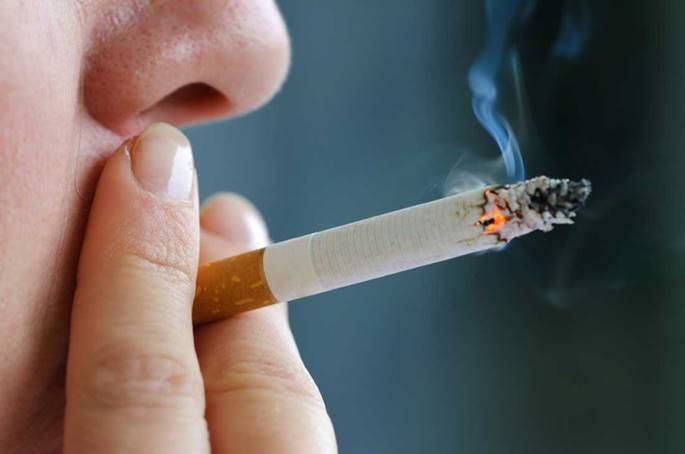
\includegraphics[width=1.00\textwidth]{les-6-smoking.jpg}
      \end{figure}
      
    \end{column}
    \begin{column}{0.7 \textwidth}
      
      \begin{itemize}
        \item \dots slechts $\frac{84}{ 24354} \times 100 = 0.35\% $ van de Britse artsen aan longkanker overleden
        \item \dots met slechts $\frac{83}{21261} \times 100 = 0.39\%$ van de rokers onder hen
        \item \dots maar  is wel  meer dan hetzelfde cijfer voor de niet-rokers $\frac{1}{3093} * 100 = 0.032\%$.
      \end{itemize}
    \end{column}
  \end{columns}
\end{frame}

\begin{frame}
  \frametitle{Rokersonderzoek}
  % Please add the following required packages to your document preamble:
  % \usepackage{booktabs}
  \begin{table}[h]
    \begin{tabular}{@{}lllll@{}}
      \toprule
      & \textbf{Longkanker} & \textbf{Niet} & \textbf{Wel} & \textbf{Totaal} \\ \midrule
      Roker & Wel                 & 21188         & 73.3         & 21261           \\
      & Niet                & 3082.3        & 10.7         & 3093            \\
      & Totaal              & 24270         & 84           & 24354           \\ \bottomrule
    \end{tabular}
  \end{table}
  
  \begin{columns}
    \begin{column}{0.3 \textwidth}
      
      \begin{figure}
        \centering
        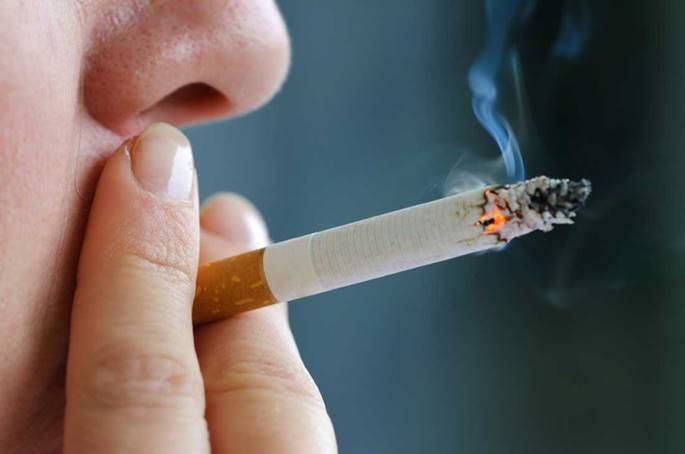
\includegraphics[width=1.00\textwidth]{les-6-smoking.jpg}
      \end{figure}
      
    \end{column}
    \begin{column}{0.7 \textwidth}
      
      \begin{itemize}
        \item $\chi^{2} = 10.35$
        \item We zien in de tabel  dat er wel een erg groot verschil is tussen de geobserveerde aantallen rokers die overlijden aan longkanker en de verwachte waarden in deze cel.
        \item Hetzelfde geldt voor het geringe aantal huisartsen dat niet rookt, maar wel aan longkanker overleden is.
      \end{itemize}
    \end{column}
  \end{columns}
\end{frame}

\begin{frame}
  \frametitle{Rokersonderzoek}
  \begin{enumerate}
    \item \textbf{Bepalen hypotheses}
    \begin{itemize}
      \item $H_{0}$: in de populatie is er geen samenhang tussen onafhankelijke en afhankelijke variabele
      \item $H_{1}$: er bestaat wel een samenhang tussen de variabelen in de populatie
    \end{itemize}
    \item \textbf{Bepalen $\alpha$ en $n$} : $\alpha = 0.05$ en $n = 24354$.
    \item \textbf{Toetsingsgrootheid en waarde ervan in steekproef}:
    \[ \chi^{2} = \sum_{i=1}^{n} \frac{(o_{i} - e_{i})^{2}}{E_{i}} = 10.35 \]
    \item \textbf{Bereken en teken kritiek gebied}:  kritieke grens is 3.8415 en aantal vrijheidsgraden $df = (r-1)(k-1)$ Onze toetsingsgrootheid ligt dus in het kritieke gebied dus verwerpen we $H_{0}$.
  \end{enumerate}
\end{frame}

\begin{frame}
  \frametitle{Oorzakelijk verband}
  We moeten derhalve $H_{0}$, dat er geen relatie is tussen beide variabelen, verwerpen ten gunste van $H_{1}$ dat er wel een relatie is tussen beide variabelen: rokers sterven vaker aan longkanker dan niet-rokers.
  \begin{columns}
    \begin{column}{0.3 \textwidth}
      
      \begin{figure}
        \centering
        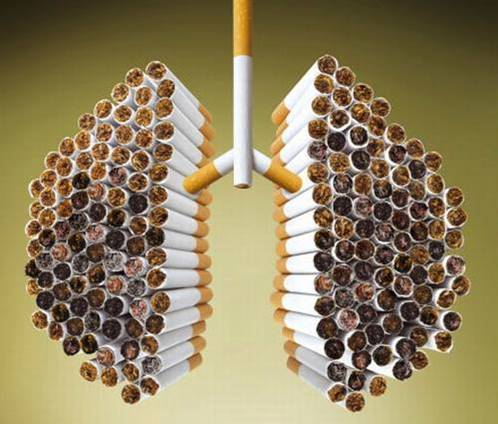
\includegraphics[width=1.00\textwidth]{les-6-smoking2.jpg}
      \end{figure}
      
    \end{column}
    \begin{column}{0.7 \textwidth}
      
      \begin{itemize}
        \item  \dots rokers zijn ouder dan de niet-rokers
        \item \dots de rokers wonen veelal in de grote steden met
        meer vervuilde lucht dan de niet-rokers
        \item \dots speciale genetische dispositie die zowel van invloed is op de verslaving aan tabak, als op de kans om longkanker te krijgen.
      \end{itemize}
    \end{column}
  \end{columns}
  Voor een causale interpretatie van de gegevens (het betreft hier immers geen experiment), moeten we op zijn minst de beschikking hebben over een theorie die de relatie tussen roken en longkanker expliciteert.
  
\end{frame}

\section{Grafieken voor kruistabellen}

\begin{frame}
  \frametitle{Visualisatie van kruistabellen}
  
  \begin{figure}
    \centering
    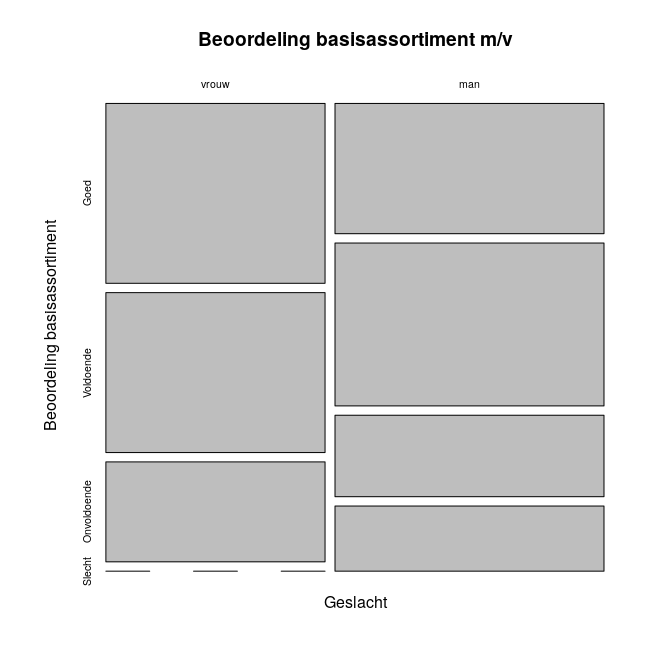
\includegraphics[height=.8\textheight]{2var-xtab-plot-waardering}
  \end{figure}
  
\end{frame}

\begin{frame}
  \frametitle{Visualisatie van kruistabellen}
  \framesubtitle{Geclusterde staafgrafiek}
  
  \begin{figure}
    \centering
    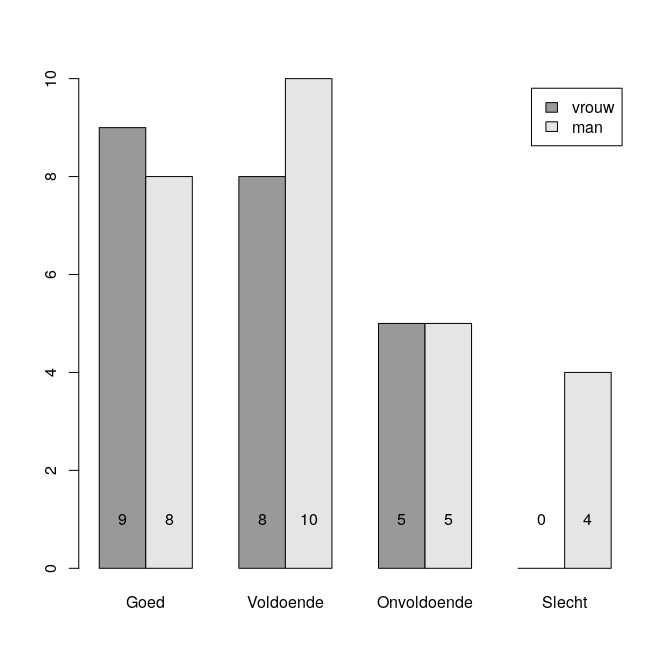
\includegraphics[height=.8\textheight]{2var-staafgrafiek-geclusterd}
  \end{figure}
  
\end{frame}

\begin{frame}
  \frametitle{Visualisatie van kruistabellen}
  \framesubtitle{Rependiagram}
  
  \begin{figure}
    \centering
    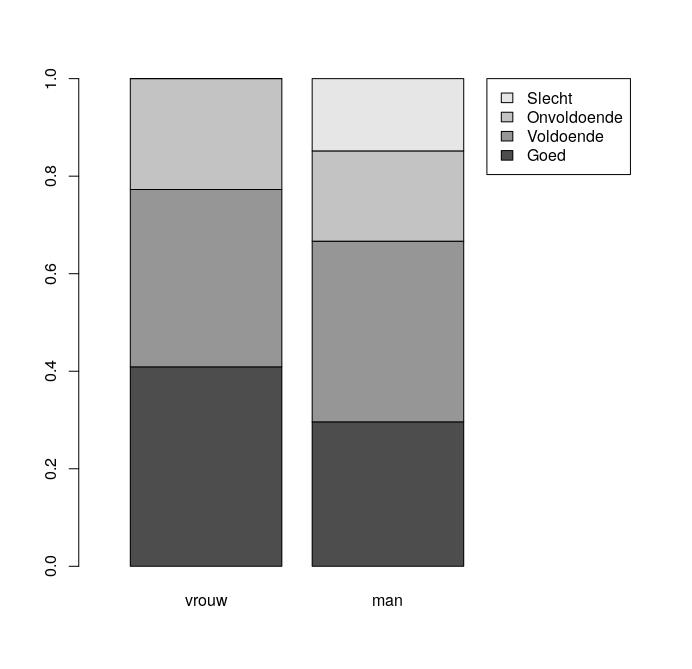
\includegraphics[height=.8\textheight]{2var-rependiagram-waardering-mv}
  \end{figure}
  
\end{frame}

\end{document}